\documentclass{article}
\usepackage{fullpage}
\usepackage{multicol}
\usepackage{graphicx}
\usepackage{mathtools}

\begin{document}
\begin{center}
{\bf 930590352}

CSCI 243 Spring 2011 HW2
\end{center}

\begin{enumerate}

\item $w$ = Randy works hard, $d$ = is a dull boy, $j$ = get a job
 \begin{enumerate}
 \item $w$ \quad\quad Hypothesis
 \item $w \rightarrow d$ \quad Hypothesis
 \item $d$ \quad\quad Modus Ponens
 \item $d \rightarrow \neg j$ \quad Hypothesis
 \item $\neg j$ \quad\quad Modus Ponens
 \end{enumerate}

\item
 \begin{enumerate}
 \item $c(x)$ = is in this class, $j(x)$ = can program in java, $p(x)$ = can get a high-paying job
  \begin{enumerate}
  \item $\forall x(j(x) \rightarrow h(x)$ \quad Hypothesis
  \item $j(doug) \rightarrow h(doug)$ \quad  Universal Instantiation
  \item $j(doug)$ \quad Hypothesis
  \item $p(doug)$ \quad Modus Ponens
  \item $c(doug)$ \quad Hypothesis
  \item $c(doug) \land p(x)$ \quad Conjunction
  \item $\exists x (c(x) \land p(x))$ \quad Existential Generalization
  \end{enumerate}
 \item $c(x)$ = is in this class, $w(x)$ = enjoys whale watching, $o(x)$ = cares about ocean pollution
  \begin{enumerate}
  \item $\exists x(c(x) \land w(x))$ \quad Hypothesis
  \item $c(y) \land w(y)$ \quad Existential Instantiation
  \item $w(y)$ \quad Simplification
  \item $c(y)$ \quad Simplification
  \item $\forall x(w(x) \rightarrow o(x))$ \quad Hypothesis
  \item $w(x) \rightarrow o(x)$ \quad Universal Instantiation
  \item $o(y)$ \quad Modus Ponens
  \item $c(y) \land o(y)$ \quad Conjunction
  \item $\exists x(c(x) \land o(x))$ \quad Existential Generalization
  \end{enumerate}
 \item $c(x)$ = is in this class, $p(x)$ = owns a PC, $w(x)$ = can use a word program
  \begin{enumerate}
  \item $\forall x(c(x) \rightarrow p(x))$ \quad Hypothesis
  \item $c(Zeke) \rightarrow p(Zeke)$ \quad Universal Instantiation
  \item $c(Zeke)$ \quad Hypothesis
  \item $p(Zeke)$ \quad Modus Ponens
  \item $\forall x(p(x) \rightarrow w(x))$ \quad Hypothesis
  \item $p(Zeke) \rightarrow w(Zeke)$ \quad Universal Instantiation
  \item $w(Zeke)$ \quad Modus Ponens
  \end{enumerate}
 \item $j(x)$ = is in NJ, $o(x)$ = within 50 miles of the ocean, $s(x)$ = has seen the ocean
  \begin{enumerate}
  \item $\exists x(j(x) \land \neg s(x))$ \quad Hypothesis
  \item $j(y) \land \neg s(y)$ \quad Existential Instantiation
  \item $j(y)$ \quad Simplification
  \item $\neg s(y)$ \quad Simplification
  \item $\forall x(j(x) \rightarrow f(x))$ \quad Hypothesis
  \item $j(y) \rightarrow f(y))$ \quad Universal Instantiation
  \item $f(y)$ \quad Modus Ponens
  \item $f(y) \land \neg s(y))$ \quad Conjunction
  \item $\exists x(f(x) \rightarrow \neg s(x))$ \quad Existential Generalization
  \end{enumerate}
 \end{enumerate}

\item 
 \begin{enumerate}
 \item False, because they imply that the conclusionmakes the begnning true.
 \item True, modus tollens is used.
 \item False, because they have $\neg p$ implying $\neg q$ which cannot be done.
 \end{enumerate}

\item 
 \begin{enumerate}
 \item if $n$ is odd \\
  $n=2k+1$ $\implies$ $n^3+5$ \\
  $= (2k+1)^3+5$ \\
  $= 8k^3+12k^2+6k+6$ \\
  $= 2(4k^3+6k^2+3k+3)$ \\
  thus $n^3+5$ is even
 \item if n is odd \\
  $n^3$ will be odd, but adding $5$ will make the equation so that odd + odd = even.
 \end{enumerate}

\item Prove Using Contrapossitve \\
 if $n$ is even $\implies n = 2k$ \\
 $5n+6 = 10k+6$ \\
 $5n+6 = 2(5k+3)$ \\
 Thus, $5n+6$ is even

\item Prove by Exhaustion \\
 $n > 4 \implies n^3 >100$ \\
 when n = 1,2,3,4 becuase only these are $n^3 >100$, $n^2 + n^3 = 100$ is never true. 

\item
 \begin{enumerate}
 \item 
  \includegraphics[width = .5 \textwidth] {Q7A_drawings}
 \item
  \includegraphics[width = .5 \textwidth] {Q7B_drawings} 
 \end{enumerate}

\item
 \begin{enumerate}
 \item Yes
 \item No, first has 1 element, while the second set has 2 elements.
 \item No, first set has no elements, second set has 1 element.
 \end{enumerate} 

\item
 \includegraphics[width = .3 \textwidth] {Q9}

\item One set is a 3-tuple, the other set is a 2-tuple and a 1-tuple. Therefore they are not the equivalent.

\item
 \begin{enumerate}
 \item
  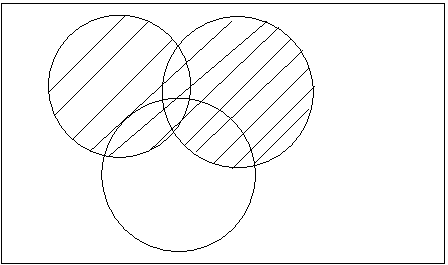
\includegraphics[width = .3 \textwidth] {Q11A}
 \item
  \includegraphics[width = .3 \textwidth] {Q11B}
 \item
  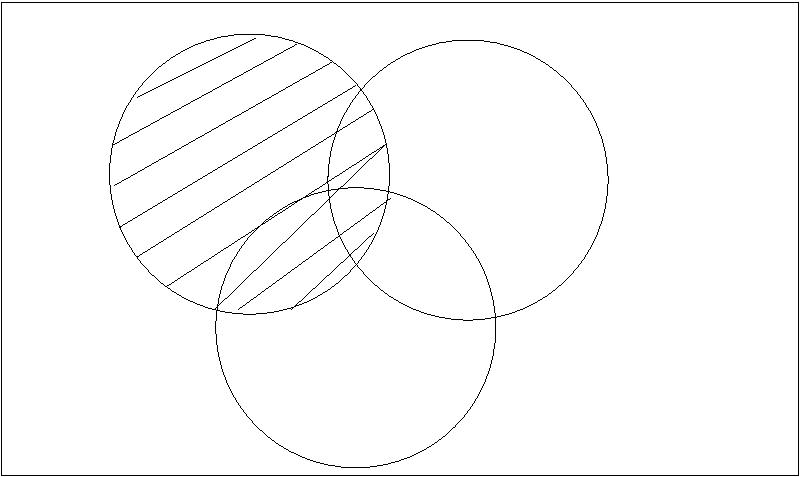
\includegraphics[width = .3 \textwidth] {Q11C}
 \end{enumerate}

\item
 \begin{enumerate}
 \item $\cup _{i=1}^{\infty}$ $A_i = Z$ \\
       $\cap _{i=1}^{\infty}$ $A_i = \{-1,0,1\}$ 
 \item $\cup _{i=1}^{\infty}$ $A_i = Z - \{0\}$ \\
       $\cap _{i=1}^{\infty}$ $A_i = \emptyset$ 
 \item $\cup _{i=1}^{\infty}$ $A_i = R$ \\
       $\cap _{i=1}^{\infty}$ $A_i = [-1,1]$ 
 \item $\cup _{i=1}^{\infty}$ $A_i = [1,\infty)$ \\
       $\cap _{i=1}^{\infty}$ $A_i = \emptyset$ 
 \end{enumerate} 

\item
 \begin{enumerate}
 \item $f(x) = x+3$ \\
       *I got this wrong because I didn't know that I could split up to create a system of equations.  I should have set anything less than 0 to one equation and anything greater than 0 to another.
 \item $f(x)=|x|+1$
 \item
  \[
	f(x) = \left\{
	\begin{array}{l l}
	$x+1$ & \quad if x \geq 0 \\
	$|x|$ & \quad if x < 0
	\end{array} \right.
  \]
 \item $f(x) = 1$
 \end{enumerate}

\item
 \begin{enumerate}
 \item Since f is one-to-one and onto, whatever g sends into f, the resulting output will have to be one-to-one or onto. It does not matter what g sends f, f will output something that follows its properties.
 \item Since as before, whatever g sends f, the output will still be onto; no matter what the initial input is.
 \end{enumerate}

\item
 \begin{enumerate}
 \item $a_0 = 2, a_1 = 3, a_2 = 5, a_3 = 9$
 \item $a_0 = 1, a_1 = 4, a_2 = 27, a_3 = 256$
 \item $a_0 = 0, a_1 = 0, a_2 = 1, a_3 = 1$
 \item $a_0 = 0, a_1 = 1, a_2 = 2, a_3 = 3$
 \end{enumerate}

\item
 (a) each set adds one more 1 and one more 0 with each reiteration of the pattern: 1,1,1... \\
 (c) every even index has $2^n$ where n increases $2^{(\frac{n-1}{2})}$ only every other index: 32, 0, 64... \\
 (e) subtract 7 each time, 22-7n: -34, -41, -48... \\
 (g) the equation is $2n^3$: 1024, 1458, 2000...

\item 
 (a) $2+3+4+5+6= 20$  \\
 (b) $1-2+4-8+16= 11$

\item
 (a) $\frac{3(2^9-1)}{2-1} = 1533$ \\
 (b) $\frac{(2^9-1}{2-1} -1 = 510$ 

\item
 (c) $(1+1+1)+(2+2+2)+(3+3+3)=18$ \\
 (d) $(0+0+0)+(1+2+3)+(2+4+6)=18$

\item
 \begin{enumerate}
 \item Countable: $f(x)= |x|$
 \item Countable: $f(x) = x when even$ \\
                  $f(x) = 1-x when odd$
 \item Not Countable
 \item Countable: ??? \\
   *I really did not know the correspondance, but now I understand the equation is a lot like (b) but with different constants. I definitely over-thought this one.
 \end{enumerate}

\item If A is not countable within B, then a part of B is not countable, thus all are uncountable.

\end{enumerate}
\end{document}
